\documentclass[a4]{article}
\usepackage{geometry}
\geometry{verbose,tmargin=2.5cm,bmargin=2.5cm,lmargin=3cm,rmargin=3cm}
\usepackage{amsmath,amssymb,amsthm}
\usepackage{graphicx}
\graphicspath{{graphics/}}
\usepackage[utf8]{inputenc}
\usepackage{fancyvrb}
\usepackage{hyperref}
\usepackage{lscape}
\usepackage{adjustbox}
\usepackage{verbatim}
\usepackage{placeins}

\title{MultiFEBE \\ Tutorial 3: harmonic analysis of an elastic cube with boundary elements}
\author{\'A.G. Vega-Artiles}
\date{June 2022}

\begin{document}

\maketitle

\tableofcontents 

\section{Problem description}

In this third tutorial, a harmonic analysis of an elastic cube is performed using the Boundary Element Method (BEM), i.e. boundary elements. Figure \ref{fig:cube} shows the geometry. Required material and geometric properties are the Young's modulus $E$, the Poisson's ratio  $\nu$, the density $\rho$, shear modulus $\mu$, hysteretic damping $\xi$, the cube side length $L$ and the harmonic load $P$. Load $P$ can be regarded as a P-wave. Self-weight is not considered. 

The analytical solution to this problem can be obtained by means of the following equations:

\begin{equation}
	\begin{array}{l}
		k = \omega/c \\
		c_p = \mathrm{Re(c_p)}\cdot\sqrt{1+2\mathrm{i}\xi} \\
		\mathrm{Re(c_p)} = \sqrt{(\lambda+2\mu)/\rho} \\
		u(x_1,\omega) = - \dfrac{\mathrm{e}^{-\mathrm{i}kx_1}-\mathrm{e}^{\mathrm{i}kx_1}}{(\lambda+2\mu)\cdot\mathrm{i}k\cdot(\mathrm{e}^{-\mathrm{i}kL}+\mathrm{e}^{\mathrm{i}kL})}
	\end{array}
\end{equation}

where natural frequencies can be calculated as:

\begin{equation}
	\centering
	\omega_n=\frac{Re(c_p)\pi}{2L}n;\quad n=1,3,5...
\end{equation}

The problem is solved for $L=1$ $\mathrm{m}$, $E=1$ $\mathrm{N/m^2}$, $\nu=0.25$, $\mu=1$ $\mathrm{N/m^2}$, $\rho=1$ $\mathrm{kg/m^3}$, $\xi=0.02$ and $P=1$ $\mathrm{N/m^2}$. First, second and third natural frequencies are: 

\begin{equation}
	\begin{array}{l}
		\omega_1 = 2.6 \medspace \mathrm{rad/s} \\
		\omega_3 = 7.7 \medspace \mathrm{rad/s} \\
		\omega_5 = 12.8 \medspace \mathrm{rad/s}
	\end{array}
\end{equation}

\begin{figure}[h]
	\centering
	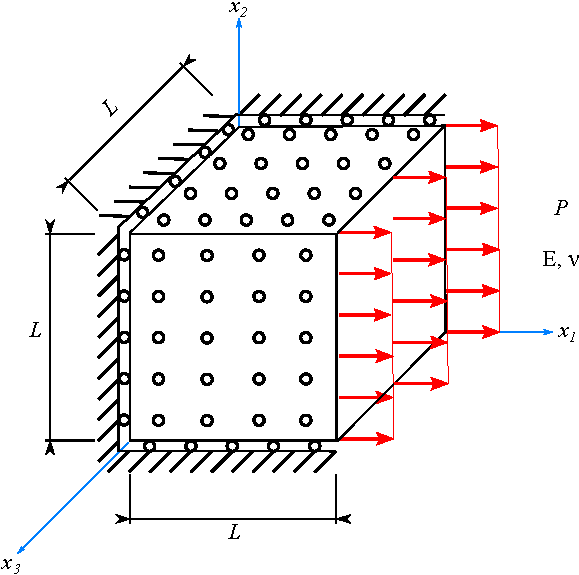
\includegraphics{cube.eps}
	\caption{Problem layout.}
	\label{fig:cube}
\end{figure}

\section{Pre-processing} 
Pre-processing in MultiFEBE consists of defining the geometry and mesh of the problem. There are three ways to do such definition: directly from the input file (mode = 0), from another file in the native format (mode = 1) or from another file in the Gmsh MSH file format version 2.2 (mode = 2), where syntax will be explained in the following subsections. Furthermore, as the problem will be solved using only the BEM formulation, the approaches explained in the previous section will be applied.      

\subsection{Gmsh format}
Gmsh \cite{gmsh, gmshweb} is a finite element mesh generator with its own language. The software allows to create the geometry in a “bottom-up” manner, going from the most basic elements (points) to the highest order elements (volumes) or in a “Constructive Solid Geometry” manner (boolean operations) or with a combination of methodologies. Gmsh also allows to define  the so-called “physical groups” which are unmodifiable entities that gather elementary entities as sole entities, where every entity must have a unique tag. On the other hand, the file containing all this geometric definition is the *.geo file whereas the mesh definition is in the *.msh file. 

\subsubsection{GEO file}
The *.geo file for this problem is the same as the one used in \emph{Tutorial 2}, but setting the element size (es) as 0.07, smaller than $\lambda/4$, and the element order as 2.

\subsubsection{MSH file}
The *.msh file for this problem is the same as the one used in \emph{Tutorial 2}, but with more nodes and elements due to the fact that the es was set as 0.07.

\begin{figure}[h]
	\centering
	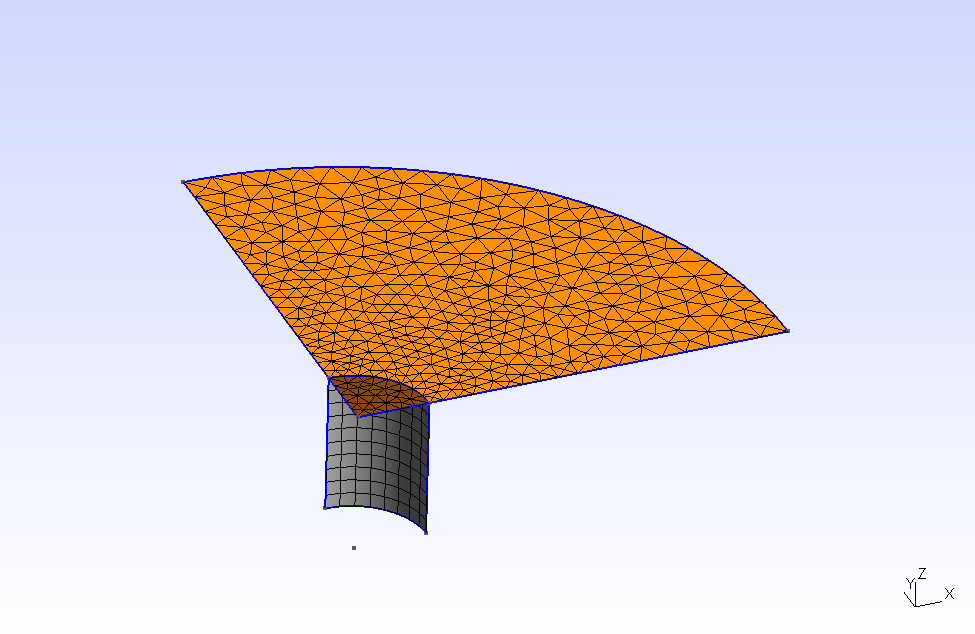
\includegraphics[scale = 0.3]{mesh.png}
	\caption{Mesh from the *.msh file.}
	\label{fig:mesh}
\end{figure}

\subsection{Input data file}
Solving in MultiFEBE consists of running the software by specifying several options in the following sections\footnote{See reference manual.}: [problem], [settings], [materials], [boundaries], [regions] and [conditions over the boundaries].

The first part to configurate is the problem definition in the section [problem]. This example is a 3D harmonic mechanical problem.  

\begin{Verbatim}	
[problem]
n = 3D
type = mechanics
analysis = harmonic
\end{Verbatim}

Then, a list of frequencies is generated by specifying the number of frequencies, that must be $\geq 2$, (300), followed by the minimum frequency, $>$ 0, ($0.01$) and the maximum frequency ($15.$), being each one in new lines.

\begin{Verbatim}
[frequencies]
rad/s
lin
300
0.01
15.
\end{Verbatim}

Next step is to configurate the mesh. In this case, a mesh from Gmsh will be used so that it is necessary to write the option number 2 and the document name obtained from it in the section [settings]. However, if the mesh were going to be read from the input file, it would require to write the sections [nodes], [elements] and [parts] instead.

\begin{Verbatim}	
[settings]
mesh_file_mode = 2 "t3.msh"
\end{Verbatim}

As the problem has just one material, the section [materials] will need two lines: a first line for the number of materials in the model and a second line for the properties such as tag, type, $\rho$, $\mu$, $\nu$ and $\xi$.

\begin{Verbatim}	
[materials]
1
1 elastic_solid rho 1. mu 1. nu 0.2 xi 0.02
\end{Verbatim}

In the section [boundaries], it is necessary to specify the number of boundaries in the first line and a line per boundary by indicating the boundary identifier, the identifier of the part that discretizes it, and finally the boundary class. In this example there are 6 boundaries: boundary 1 is the part 1 of the mesh, boundary 2 the part 2, boundary 3 the part 3, boundary 4 the part 4, boundary 5 the part 5 and boundary 6 the part 6 and all of them are ordinary boundaries.

\begin{Verbatim}	
[boundaries]
6
1 1 ordinary
2 2 ordinary
3 3 ordinary
4 4 ordinary
5 5 ordinary
6 6 ordinary
\end{Verbatim}

The format of the section [regions] consists of a first line indicating the number of regions (1). Furthermore, for each region there must be a block of data consisting of several lines of data. The first one is the region identifier and the region class (discretization method) (1 be). As the region is a BE region, then the second line indicates the number and list of boundaries (6 1 2 3 4 5 6). The third line defines the material (material 1). Then, for a BE region, the fourth line defines the number and list of BE body loads (0) and the fifth line the number and list of incident fields (0).

\begin{Verbatim}	
[regions]
1

1 be
6 1 2 3 4 5 6
material 1
0
0
\end{Verbatim}

In the section [conditions over be boundaries], all boundaries will be specify in global coordinates because they are planar and their normal vectors are parallel to one of the global axes. As a 3D problem, there are three lines for every boundary: a first line for the x direction, the second one for the y direction and the third one for the z, where the first number of every line indicates the type of condition (here 0 for displacement and 1 for traction) and the second one its value in complex number because it is a harmonic analysis.

\begin{Verbatim}	

[conditions over be boundaries]
boundary 1: 1 (0.,0.)
            1 (0.,0.)
            0 (0.,0.)

boundary 2: 1 (1.,0.)
            1 (0.,0.)
            1 (0.,0.)

boundary 3: 1 (0.,0.)
            1 (0.,0.)
            0 (0.,0.)

boundary 4: 0 (0.,0.)
            0 (0.,0.)
            0 (0.,0.)

boundary 5: 1 (0.,0.)
            0 (0.,0.)
            1 (0.,0.)

boundary 6: 1 (0.,0.)
            0 (0.,0.)
            1 (0.,0.)
\end{Verbatim}

The whole script applied to the problem is the following:

\begin{Verbatim}
[problem]
n = 3D
type = mechanics
analysis = harmonic

[frequencies]
rad/s
lin
300
0.01
15.

[settings]
mesh_file_mode = 2 "t3.msh"

[materials]
1
1 elastic_solid rho 1. mu 1. nu 0.2 xi 0.02

[boundaries]
6
1 1 ordinary
2 2 ordinary
3 3 ordinary
4 4 ordinary
5 5 ordinary
6 6 ordinary

[regions]
1

1 be
6 1 2 3 4 5 6
material 1
0
0

[conditions over be boundaries]
boundary 1: 1 (0.,0.)
            1 (0.,0.)
            0 (0.,0.)

boundary 2: 1 (1.,0.)
            1 (0.,0.)
            1 (0.,0.)

boundary 3: 1 (0.,0.)
            1 (0.,0.)
            0 (0.,0.)

boundary 4: 0 (0.,0.)
            0 (0.,0.)
            0 (0.,0.)

boundary 5: 1 (0.,0.)
            0 (0.,0.)
            1 (0.,0.)

boundary 6: 1 (0.,0.)
            0 (0.,0.)
            1 (0.,0.)
\end{Verbatim}

\section{Results and discussion}

\subsection{Nodal solutions file (*.nso)}
The results of a node from the face $x_1=L$ for $es=1$ and $es=0.07$ was taken and plotted together with the analytical solution to observe the frequency response in Figure \ref{fig:cube_results} and Figure \ref{fig:cube_results2}.

It can be seen that the numerical solution for $es=0.07$ is in perfect agreement with the analytical solution but there are discrepancies for $es=1$.

\begin{figure}[h]
	\centering
	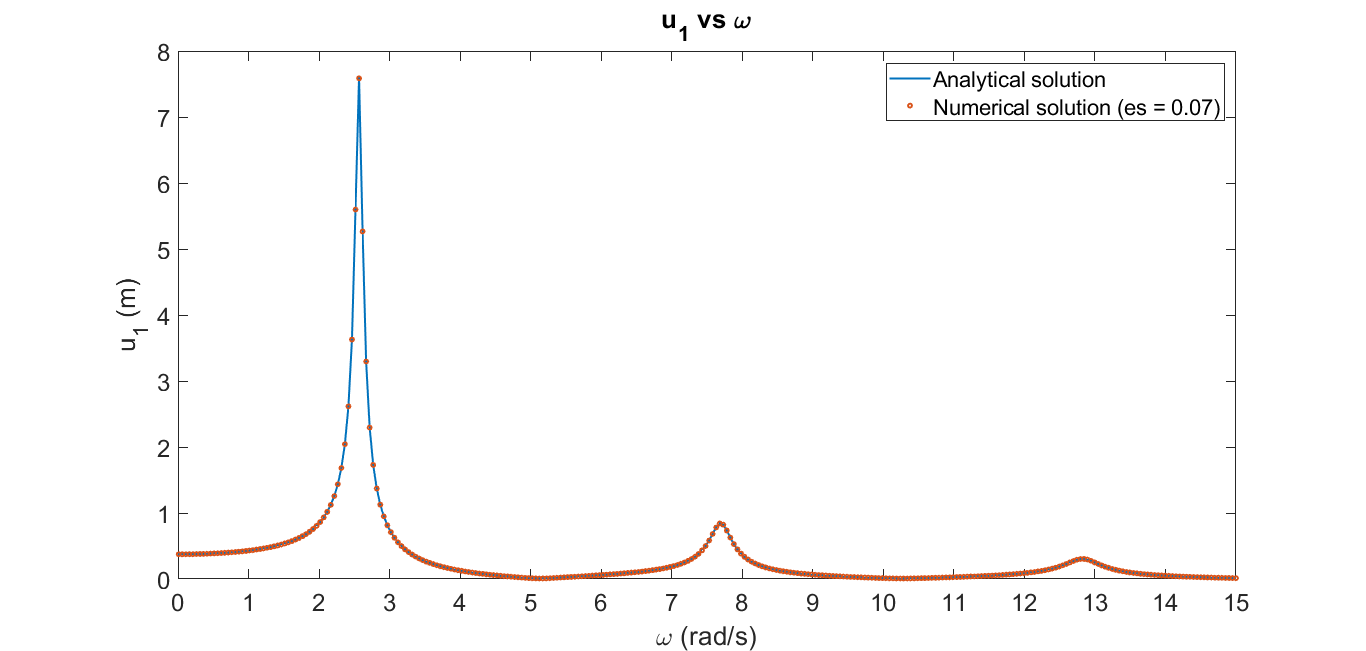
\includegraphics[scale = 0.45]{es007.png}
	\caption{Results of the harmonic elastic cube (es = 0.07).}
	\label{fig:cube_results}
\end{figure}

\begin{figure}[h!]
	\centering
	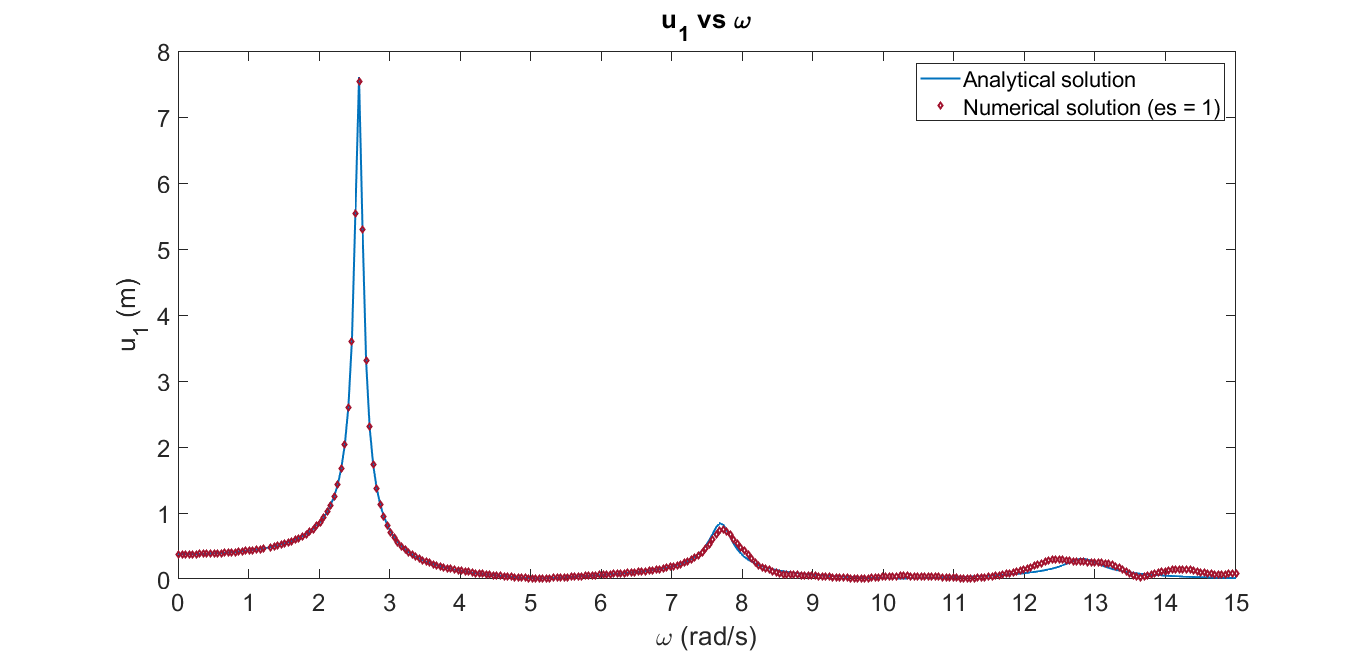
\includegraphics[scale = 0.45]{es1.png}
	\caption{Results of the harmonic elastic cube (es = 1).}
	\label{fig:cube_results2}
\end{figure}

\subsection{Gmsh results file (*.pos)}

The file for the current example is the following:

\begin{figure}[h]
	\centering
	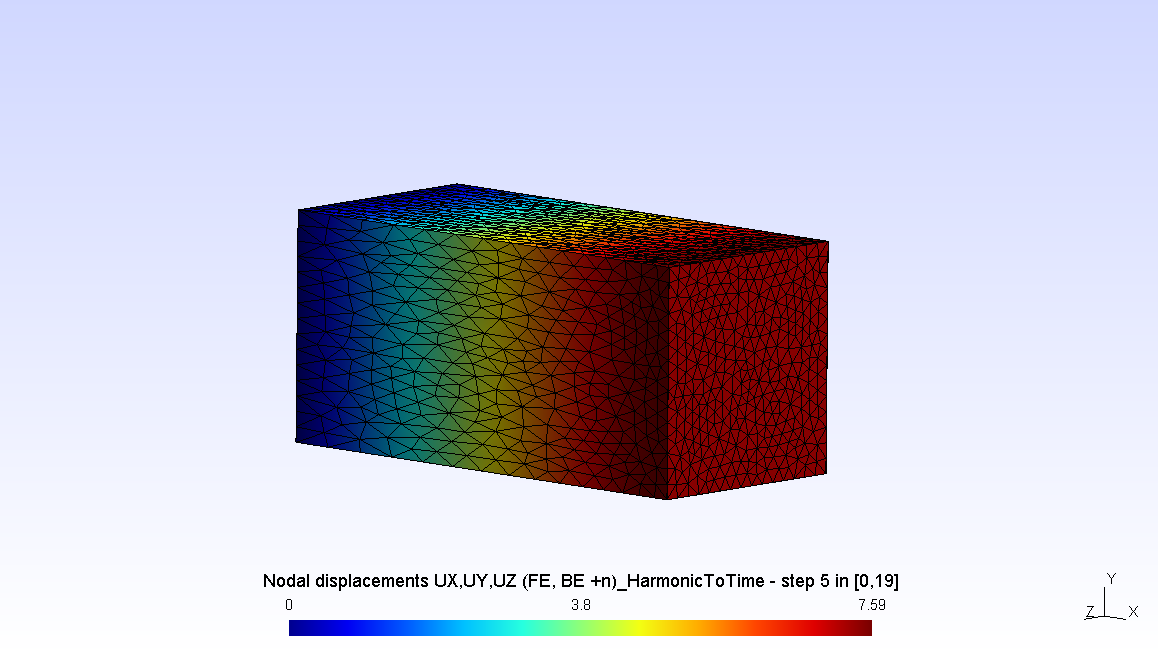
\includegraphics[scale = 0.5]{u_w1.png}
	\caption{Nodal displacement results for $\omega_1$ with a displacement factor of 0.15 from the *.pos file.}
	\label{fig:u_w1}
\end{figure}

\begin{figure}[h!]
	\centering
	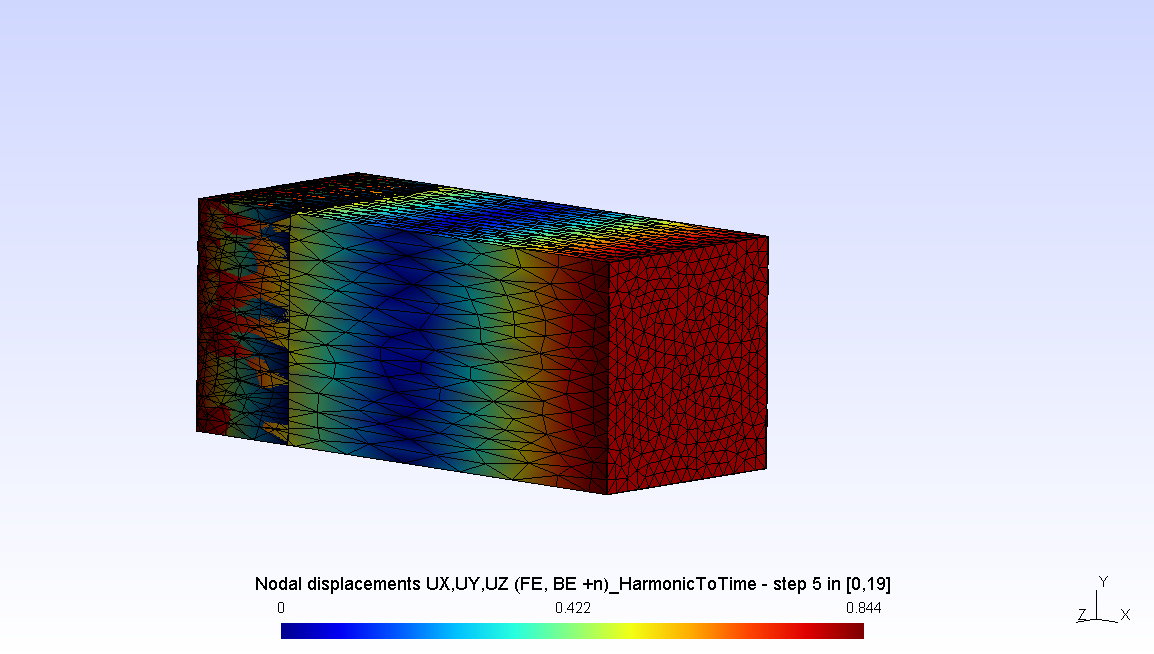
\includegraphics[scale = 0.5]{u_w3.png}
	\caption{Nodal displacement results for $\omega_3$ from the *.pos file.}
	\label{fig:u_w3}
\end{figure}

\begin{figure}[h!]
	\centering
	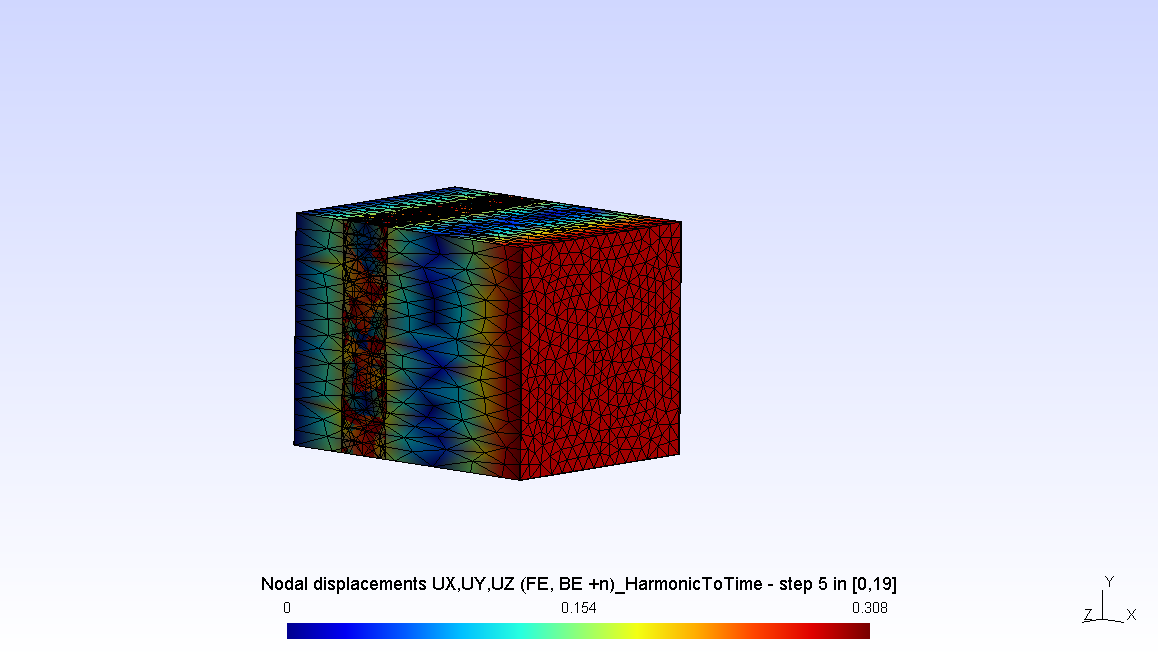
\includegraphics[scale = 0.5]{u_w5.png}
	\caption{Nodal displacement results for $\omega_5$ from the *.pos file.}
	\label{fig:u_w5}
\end{figure}

\FloatBarrier

\begin{thebibliography}{99}
	
	\bibitem{gmsh} C. Geuzaine and J.-F. Remacle, ``Gmsh: a three-dimensional finite element mesh generator with built-in pre- and post-processing facilities." \textit{International Journal for Numerical Methods in Engineering}, Volume 79, Issue 11, pages 1309--1331, (2009).
	
	\bibitem{gmshweb}  C. Geuzaine and J.-F. Remacle, ``Gmsh." \url{http://gmsh.info/}
	
\end{thebibliography}

\end{document}
